%!TEX root = report.tex

\chapter{Discussion and Future Work}

In this chapter we first discuss the experiments and their results. Then we
proceed to discuss the model based on experiments. Finally, we present some
thoughts on interesting research opportunities.

\section{Discussion of results}

In this section we will comment on the results obtained, primarily from our
experiments. More importantly, we will also expand upon the discussion
presented for each experiment in the Chapter 4 where we explained our
experimental approach.

\subsection{Experiment 1: Wireshark}

As revealed in Figure \ref{fig:wstiming} (actual timing model), the design of
this experiment has a critical flaw which is not apparent without deeper
insight into the network stack. As explained earlier, the ``packet tap''
feature from which Wireshark obtains packets is triggered when the packet
exits the kernel queueing system (qdisc) and handed over to the driver for
transmission, rather than once the driver receives a transmission event from
the hardware. This completely invalidates the fundamental design model and
thus the experiment as such.

Further exploration showed that the experiment design could work if packets
could be timestamped in hardware and somehow captured after transmission.
There \emph{is} support for this in Linux, and Wireshark, but unfortunately
relies on features not available in our hardware.

The presented results are mostly included for completeness and should not be
regarded as anything useful, except for measuring system call to pcap
latencies.

\subsection{Experiment 2: Queueing the Network System}

As described in Section \ref{sec:experiment2}, there are some issues with the
definition of $W_\text{NIC}$ from Equation \ref{eq:wnic} due to a deferred
memory release mechanism in the kernel. Specifically, the definition of the
NIC queuing system from Figure \ref{fig:exp2_overview} includes a note
``kernel scheduler frees handled pkts''.

In order to increase throughput (at the expense of latency), Linux will free
up handled packets in batches. This part greatly impacts the \texttt{sndbuf}
which is used in Equation \ref{eq:sndbuf}, implying that sent or dropped
packets -- but not yet freed -- will still count as enqueued in the NIC. In
short, the modeled $L_\text{NIC}$ includes packets in driver/firmware, in
hardware and, crucially, in the kernel's to-free list.

By increasing the \texttt{sndbuf} we could observe a corresponding increase in
$L_\text{NIC}$ (and $W_\text{NIC}$) in our experiments. However, this fact
does not imply that there are not any more packets in the NIC. Recall that the
NIC queueing system actually consists of a driver/firmware queue and a
hardware queue. The hardware queue on most consumer chips is \emph{probably}
either fixed and very limited in size, or non-existant (flash memory \emph{is}
expensive).

After additional analysis of the source code of Intel's open source Wi-Fi
driver, the driver/firmware queue length was determined to be 256 packets
large. By assuming a full \texttt{sndbuf} (i.e. $K$ packets in the network
system) and a full NIC, we can model $K$ as $K = L_\text{qdisc} + 256 +
\text{hardware} + \text{to-be-free}$ where \texttt{hardware} and
\texttt{to-be-freed} are unknowns.

One can argue that for the hardware queue to have any impact on the other
queues, it would have to be of similar size. Otherwise, it should be safe to
assume an (soft)interrupt-based solution: driver manages known packets and
hardware signals which have been sent. Thus the total queue size of the NIC is
determined by the driver, in our case $256$ packets, simplifying $K =
L_\text{qdisc} + 256 + \texttt{to-be-freed}$. This exposes the core issue with
the original queue model: there is no separation between ``in queue, waiting
to be served'' and ``served, waiting to be freed''.

In the program which logged $L_\text{qdisc}$, we could observe how many
packets were fed into the driver ``at once''. Our tests show around multiple,
10+, packets being handed over to the driver. This confirms that the driver is
able to keep the internal buffer/queue fully saturated, but does not shed
any light on the size of \texttt{to-be-freed}.

With no clear understanding of the potential size of \texttt{to-be-freed}.

% TODO: explain why to-be-freed must be known for this experiment to work

% Recall Little's Law $L = \lambda W$, increasing $L$ must give a relatively
% similar increase in either the arrival rate $\lambda$ or service time $W$.
% Since the arrival rate is fixed, it must be the service time $W$. Finally,
% recall that service time includes the time a packet spends waiting in the
% queue. This was originally expressed as a time $T_\text{QUEUE}$ component. By
% splitting the NIC queue system into a cascaded driver and hardware,
% $\lambda_\text{pktgen} \rightarrow \text{driver} \rightarrow \text{hardware}
% \rightarrow \lambda_\text{xmit}$.

% $L_\text{driver} \approx 256$, then the service times of the two systems can
% be expressed as $W_\text{driver} = 256 W_\text{hardware}$, assuming that the
% driver system is a bottleneck.

% Furthermore, by assuming that $L_\text{hardware} \approx 1$, i.e. a system
% with queue length zero, all time spent in the system is due to service, which
% in the case of the hardware system exactly matches the definition of
% \emph{channel access delay}. This can be simplified further, since the arrival
% rate of a bottlenecked queueing system is equal to the service rate,
% $\lambda_\text{NIC} = \lambda_\text{pktgen} = \lambda_\text{xmit}$.

% \begin{equation}
% W_\text{hardware} = \frac{1}{\lambda_\text{hardware}} = \frac{1}{\lambda_\text{xmit}} = \frac{1}{\lambda_\text{pktgen}}
% \end{equation}

% Equation \ref{eq:wnic}, rewritten for $W_\text{hardware}$, becomes

% \begin{align}
% W_\text{hardware} =&~T_\text{DIFS} + T_\text{BACKOFF} \nonumber\\
%               &+ T_\text{PHY} + T_\text{MAC} + T_\text{FRAME}\\
%               &+ T_\text{SIFS} + T_\text{ACK}\nonumber
% \end{align}



% \item jana + qdisc + sndbuf (hacker) -- A second attempt at capturing
%   network timing statistics by modelling the Linux kernel's network system
%   as a queuing system.


%   \item TG799-vac: metrics quality -- The primary testing device provides
%   network-related statistics via \texttt{ubus}. A first due dilligence smoke test
%   was performed to reveal any significant issues with the reported data. I.e.
%   "can we trust what we get?"

%   \item TG799-vac rssi quality -- A special-case test for the reported RSSI
%   (Relative Signal Strength Indicator) metric to find any obvious errors.

%   \item Felemban-Ekici in the wild -- Map \emph{model metrics} to \emph{captured
%   metrics} from a TG799-vac using \texttt{ubus}, and evaluate against dataset
%   obtained from a production network.
% \end{itemize}

% The \emph{conditional packet collision probability} can be empirically obtained by
% finding the number of transmission collisons and transmission attempts:

% \[
%   P(\text{collision}\|\text{transmission}) = \frac{tx_{collisions}}{tx_{success}+tx_{collisions}}
% \]

% Similarly, the \emph{model metric} \emph{channel access delay} can be obtained
% by measuring the total time described in Figure \ref{fig:timings}.

\subsection{Experiment 3: Hacking on the driver}

% TODO: Discuss wireless media time, 2G and 5G difference
The presented \texttt{wireless\_media\_time} shows signs of


Recall that during the CSMA process, time is quantized into time-slots, from 9
to 50 $\mu s$. At similar physical transmission rates, with $T_{\texttt{slot}}
= 9$ will \emph{attempt} to decrement the $T_{\texttt{backoff}}$ more than 5
times as quickly, compared with $T_\texttt{slot} = 50$. However, since
transmission take exactly the same amount of time, the only difference becomes
the time spent waiting for the \texttt{DIFS} and \texttt{SIFS}. Now consider
that when $T_{\texttt{slot}} = 9$, the physical transmission rate is 200 Mbps
and 72.2 when $T_{\texttt{slot}} = 50$ -- this is IEEE 802.11 n compared to
IEEE 802.11 ac. The insight here is that a IEEE 802.11 ac network can send
frames a) faster compared to n and b) decrements the backoff counter more
rapidly, with the implication that, network-wide, there will be more
transmission attempts and, consequently, packet collisions, compared to
IEEE 802.11 n, assuming network saturation and equal sample durations.

This behavior is shown by the graphs -- the IEEE 802.11 ac frame drops is
significantly higher compared to IEEE 802.11 n. We will continue to discuss
the frame drop probability in the upcoming section.

\section{The Felemban-Ekici Model}

As it turned out, evaluating the usefulness of the Felemban-Ekici model was an
incredibly difficult endeavour. Unfortunately, the first step of the thesis --
gathering data to evaluate the model with -- turned out to be the real
challenge, and challenging problems have their own lure -- they hook you in
until they are solved, or, as in our case, time runs out.

To our disappointment, we could not discover any combination of parameters in
our re-implementation of the Felemban-Ekici model which resulted in similar
throughput and access delay results as the original paper. As seen in Figure
\ref{fig:modelimpl}, we could, however, accurately implement the conditional
packet collision $P$.

\begin{figure}[tbp]although
  \centering
  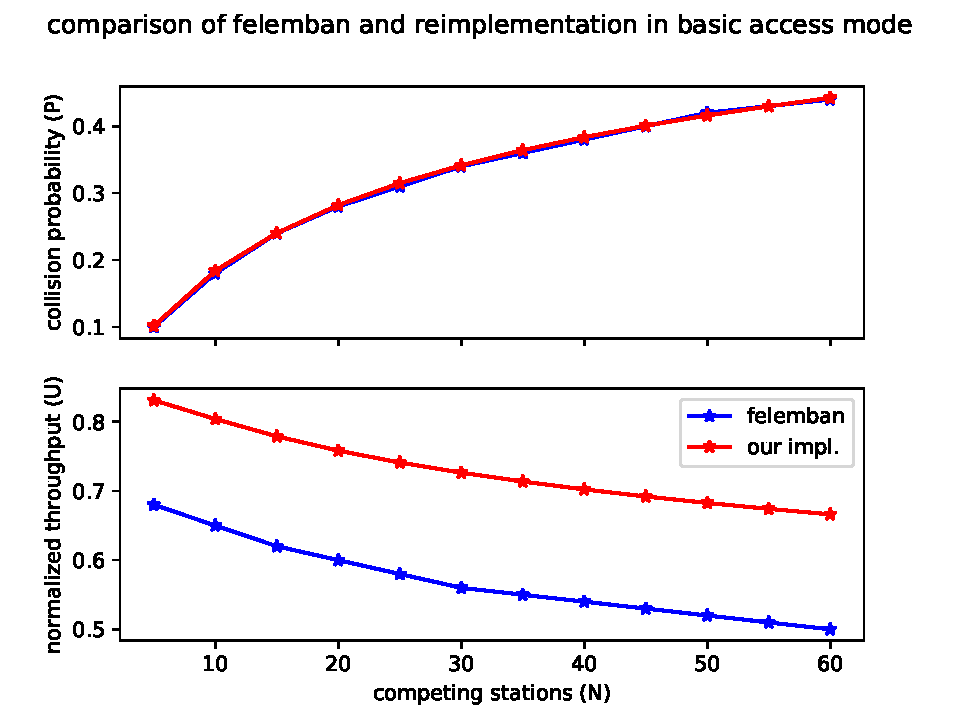
\includegraphics[width=0.8\textwidth]{images/reimpl.pdf}
  \caption{Our model reimplementation compared to values extracted from the original paper under similar network conditions.}
  \label{fig:modelimpl}
\end{figure}

To put this into perspective, at rougly 50 connected clients the conditional
packet collision probability reaches $40\%$, which results in a $0.4^{L+1}
\approx 0.06\%$ probability to fail transmission $L+1$ times and drop a
packet. At 20 clients, which is what we used during experiment 3, this falls
to $0.27^{L+1} \approx 0.003\%$.

Since clients are assumed to be identical, the packet drop probability for one
client and full network are equivalent. In Figure \ref{fig:relative_txfail_2g}
we show the total number of \texttt{tx\_fail}s (as reported to the kernel)
relative to the total number of packets transmitted, for 802.11 \emph{n}. Data
from 802.11 \emph{ac} is shown in Figure \ref{fig:relative_txfail_5g}. As seen
directly, the clients have a problem staying connected to the network throughout
the 802.11 \emph{n} test (indicated by lack of plots) and only few or no
packet drops were detected. The 802.11 \emph{ac} test, however, hovers around
the $0.003$, a full two orders of magnitude larger than the model's estimated
$0.003\%$.

\begin{figure}[tbp]
  \centering
  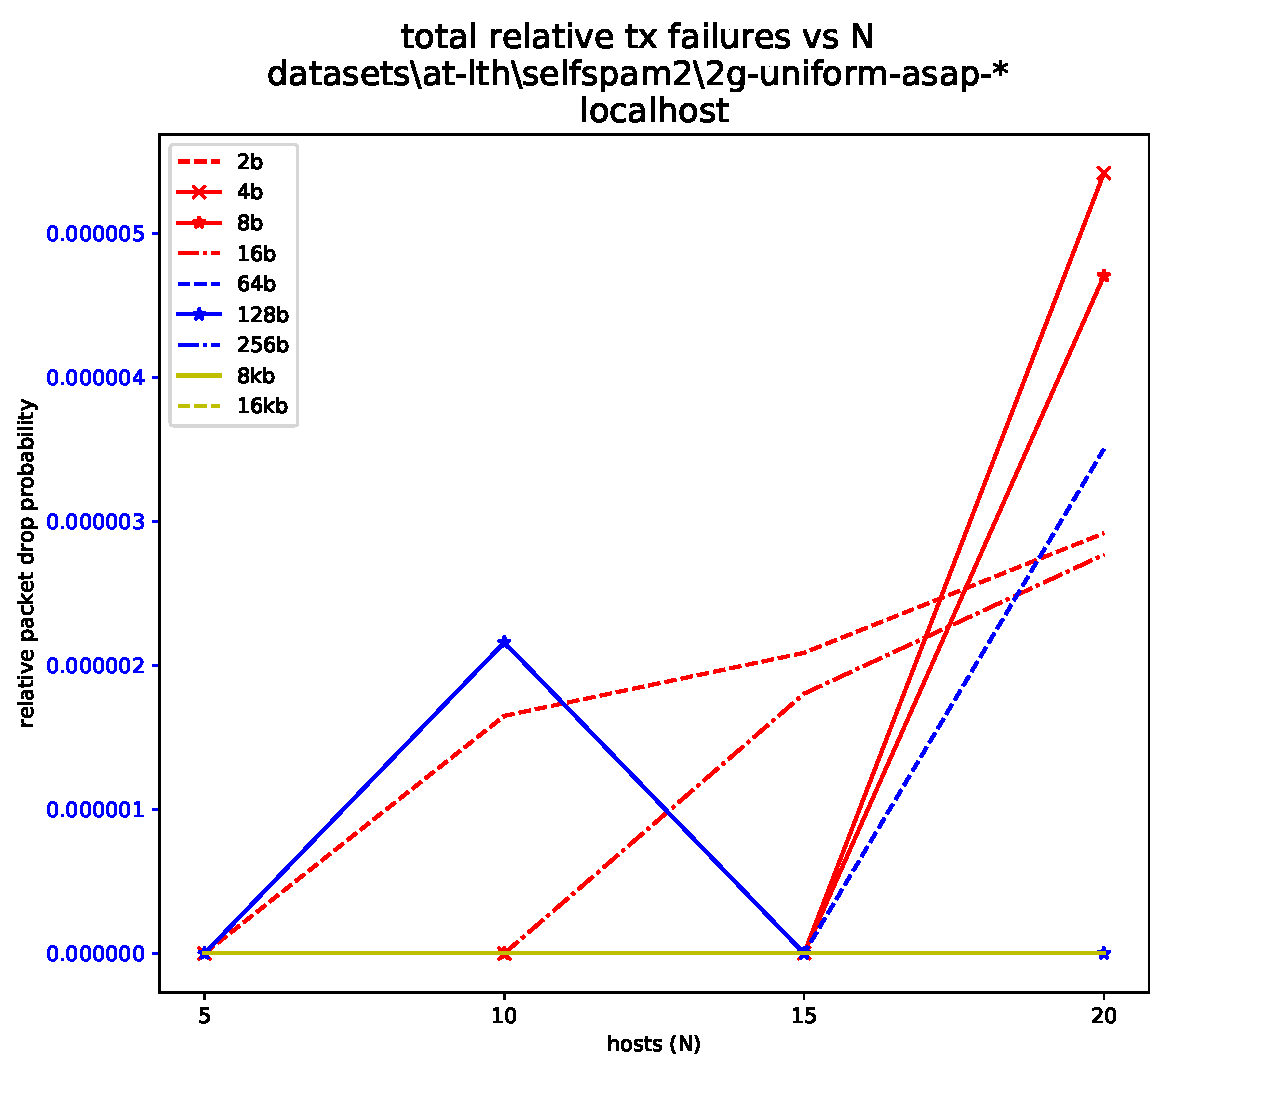
\includegraphics[width=0.8\textwidth]{images/relative_tx_fail_2g.pdf}
  \caption{Empirically obtained packet drop probability for 802.11 n.}
  \label{fig:relative_txfail_2g}
\end{figure}

\begin{figure}[tbp]
  \centering
  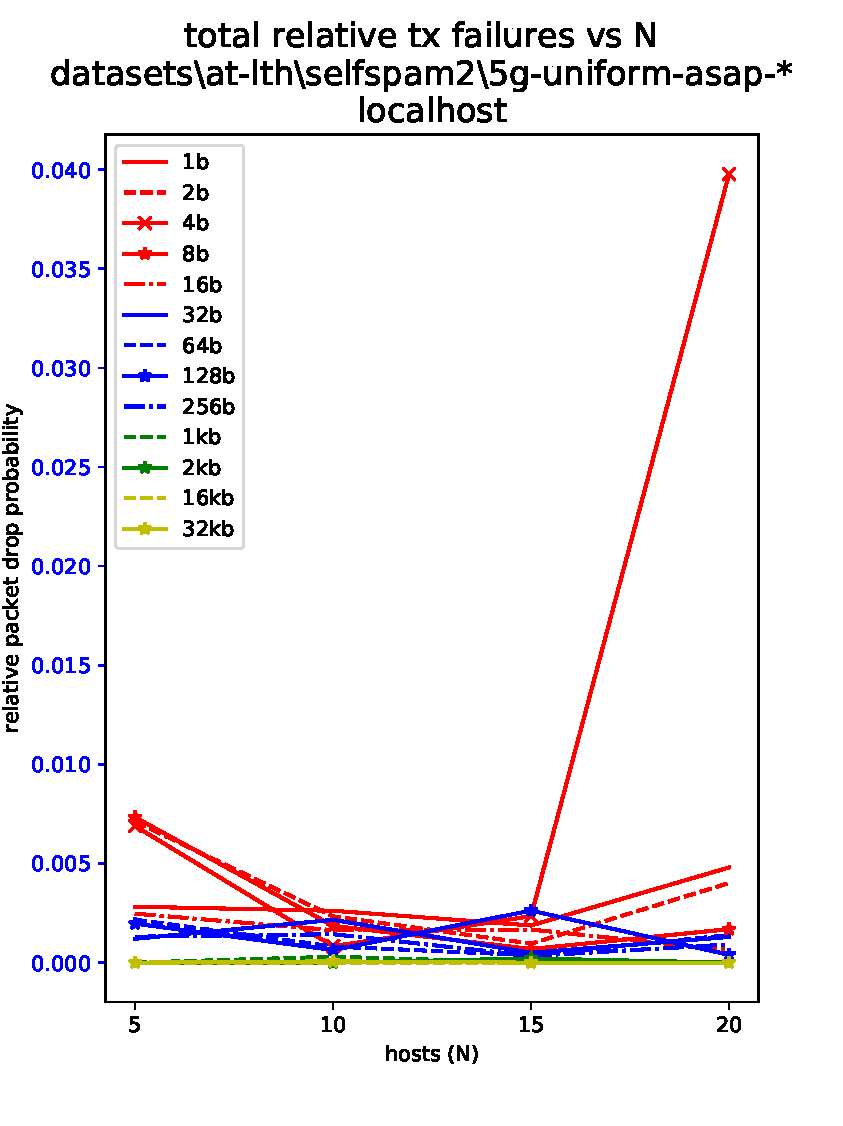
\includegraphics[width=0.8\textwidth]{images/relative_tx_fail_5g.pdf}
  \caption{Empirically obtained packet drop probability for 802.11 ac.}
  \label{fig:relative_txfail_5g}
\end{figure}

Finally, we tried to rescale and normalize the throughput by assuming that the
model was true. The model estimates about that at $N = 5$, normalized
throughput is at $68\%$, which puts channel capacity at
$\frac{\text{throughput}}{0.68}$. Figures \ref{fig:rescaled_tput_2g} and
\ref{fig:rescaled_tput_5g} show the (rescaled) normalized network throughput
(using the computed channel capacity), for varying $N$ and payload size. In
both figures, the cyan curve show the normalized throughput obtained from the
Felemban-Ekici paper with 1 KB payload at 1 Mbps (over 802.11 n).

\begin{figure}[tbp]
  \centering
  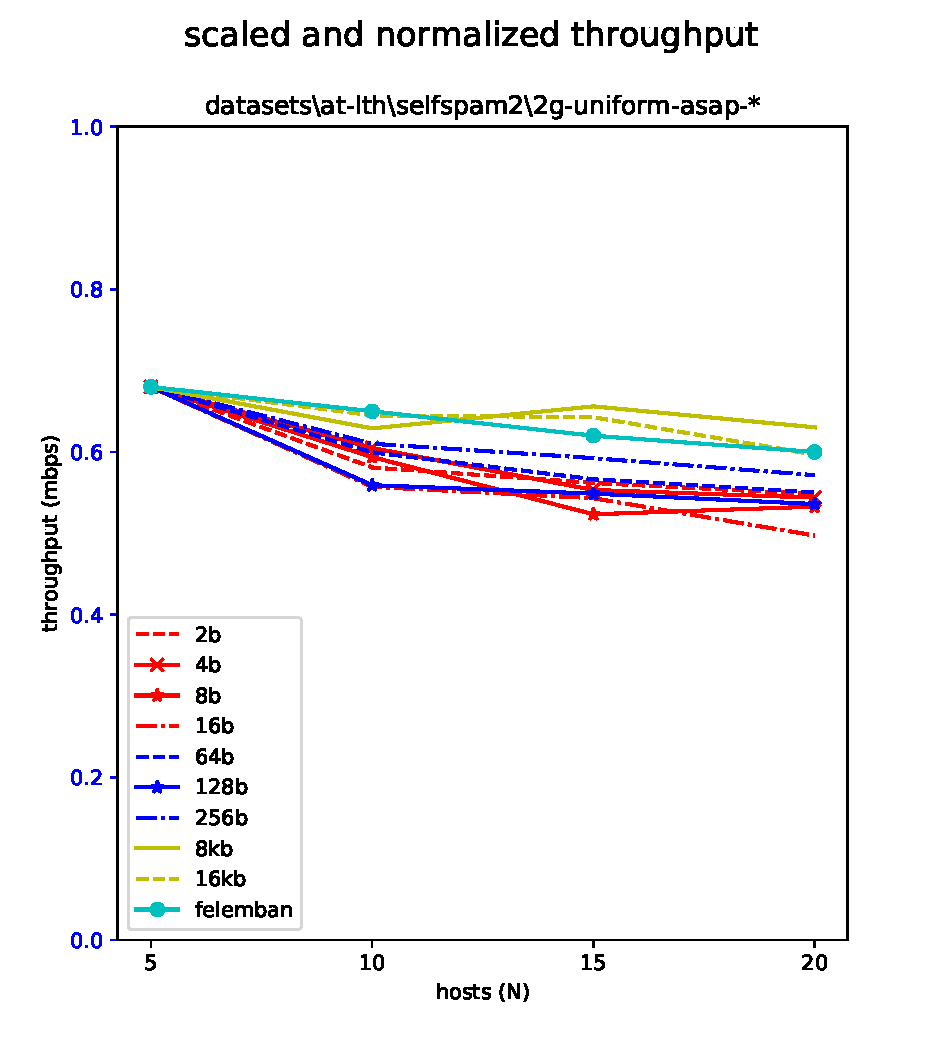
\includegraphics[width=0.8\textwidth]{images/rescaled_u_2g.pdf}
  \caption{Rescaled, (measured) normalized network throughput for 802.11 n compared with Felemban-Ekici.}
  \label{fig:rescaled_tput_2g}
\end{figure}

\begin{figure}[tbp]
  \centering
  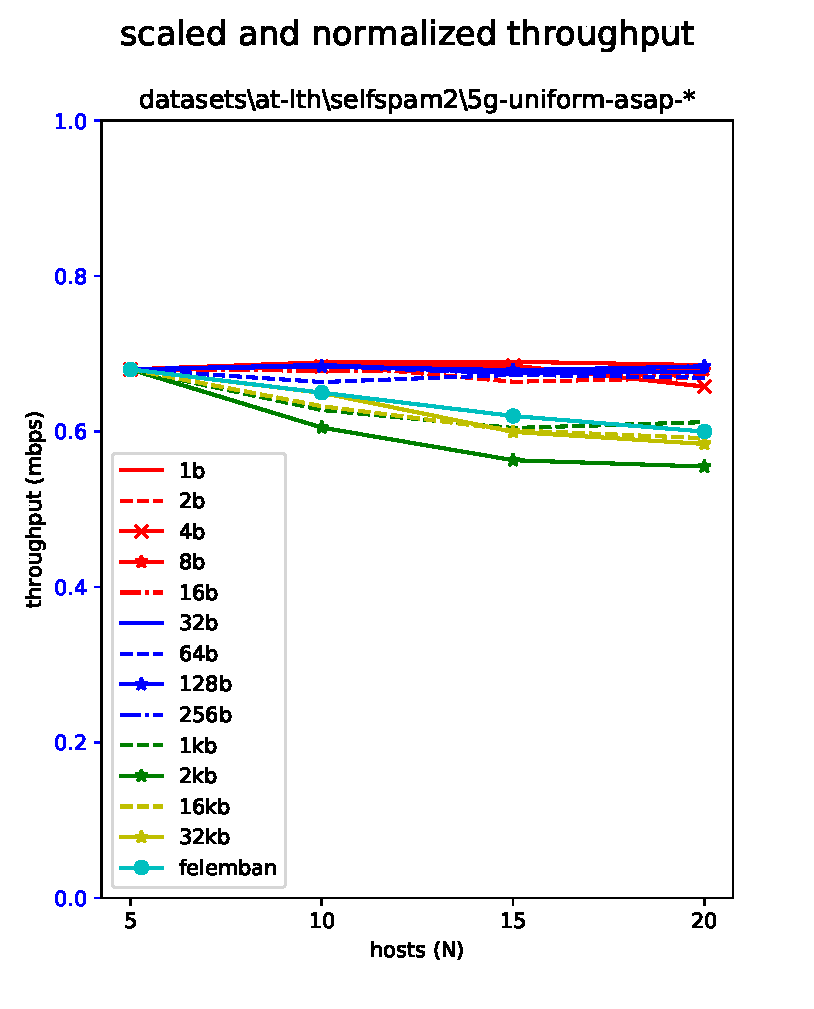
\includegraphics[width=0.8\textwidth]{images/rescaled_u.pdf}
  \caption{Rescaled, (measured) normalized network throughput during 802.11 ac compared with Felemban-Ekici.}
  \label{fig:rescaled_tput_5g}
\end{figure}

Figure \ref{fig:rescaled_tput_2g} (802.11 n) shows an expected behavior. Larger
payload sizes have higher relative utilization and roughly follow the
Felemban-Ekici curve. Lower payload sizes fall behind very fast. This hints at
a weakness in the model regarding different traffic flows.

Seemingly in opposition, Figure \ref{fig:rescaled_tput_2g} appears to imply
that smaller payload sizes incur no penalty as $N$ increases. Figure
\ref{fig:exp4throughput} reveals why, the throughput is already incredibly
low. Moving on, the larger payload sizes show similar curves compared to
802.11 n.

In conclusion, we cannot determine whether the predicted conditional packet
collision probability is correct or not. Although the model appears to predict
network throughput degredation as the number of connected nodes increase, it's
certainly not an apples to apples comparison. Our 802.11n network was mostly
stable at 72.2 (for raspberri pi 4's) and 200 Mbps on 802.11 ac, quite
different than model's 1 Mbps channel. As we could not generate normalized
throughput values from our reimplementation we cannot know what the output of
the model would have been for our network configurations.


\section{Future work}

\begin{itemize}

\item As seen in the network overview (Figure \ref{fig:linux_egress}) and
noticed during experiment 2, system call overhead and the userland/kernel
split have serious implications for latency-sensative measurements. An area
worth exploring is known as ``userland networking'' -- a technique common in
high-performance packet processing in which a userland application is allowed
exclusive access of a network device. Bypassing the kernel removes potential
bottlenecks such as context switches, memory allocation and copying,
scheduling and multithreading. In theory, this technique can reduce the number
of system calls of an application. More importantly, such an application can
design the communication between NIC and userland as a ring buffer,
eliminating the cost associated with memory allocation and deallocation
experienced in Experiment 2 (the unknown number of \texttt{to-be-freed}
packets).

\item An alternative approach to bypassing the kernel, is to bring the
userland program \emph{into} the kernel. The Berkley Packet Filter (BPF) is a
register-based filter evaluator designed for packet filtering
\cite{10.5555/1267303.1267305}. It has since been extended and redesigned
under the ``extended BPF'' (eBPF) moniker and as an in-kernel virtual machine
with filters, taps and hooks all over the kernel. In short, the eBPF machine
can run arbitrary code inside the kernel, triggered by specific events. In
theory, this should allow for more accurate measurement of the packet
transmission process.


\item Continuing on the started path with a modified Wi-Fi driver, it would be
useful to also perform similar tests where the \texttt{jana} server also has
to reply back to the clients. These tests should more closely mimic the TCP
protocol upon which most of today's networking rely. Measuring the round trip
time (RTT) of packets and comparing the measured values with a modeled RTT (
based on IEEE 802.11 and TCP), could lead to some interesting results.


\item And as is common practice today, when in doubt, throw machine learning
at the problem. While machine learning cannot enable more accurate
measurements, a machine-learning model could be trained to predict network
behaviour based on a large set of collected and labeled (as in, metric X
indicate outcome Y) metrics. A model may also be constructed for determining
possible user-friendly interventions (move device closer to router, the
channel is currently observing heavy interference so switch channel), however
an expert system (guided by real-time metrics) would probably be sufficient.
The system could be designed to run on each device (distributed) or on a
trusted machine (centralised). A centralised machine would have more
information to act on when issuing interventions back to users and,
potentially, directly to the Wi-Fi routers. Such a system could easily be
extended to record the outcome of such interventions (e.g. significantly
better or worse), possibly allowing for collection of data for unsupervised
machine learning.

\end{itemize}
